%%%%%%%%%%%%%%%%%%%%%%%%%%%%%%%%%%%%%%%%%%%%%%%%%%%%%%%%%%%%%%%%%%%%%%%%%%%%%%%%
% Template for USENIX papers.
%
% History:
%
% - TEMPLATE for Usenix papers, specifically to meet requirements of
%   USENIX '05. originally a template for producing IEEE-format
%   articles using LaTeX. written by Matthew Ward, CS Department,
%   Worcester Polytechnic Institute. adapted by David Beazley for his
%   excellent SWIG paper in Proceedings, Tcl 96. turned into a
%   smartass generic template by De Clarke, with thanks to both the
%   above pioneers. Use at your own risk. Complaints to /dev/null.
%   Make it two column with no page numbering, default is 10 point.
%
% - Munged by Fred Douglis <douglis@research.att.com> 10/97 to
%   separate the .sty file from the LaTeX source template, so that
%   people can more easily include the .sty file into an existing
%   document. Also changed to more closely follow the style guidelines
%   as represented by the Word sample file.
%
% - Note that since 2010, USENIX does not require endnotes. If you
%   want foot of page notes, don't include the endnotes package in the
%   usepackage command, below.
% - This version uses the latex2e styles, not the very ancient 2.09
%   stuff.
%
% - Updated July 2018: Text block size changed from 6.5" to 7"
%
% - Updated Dec 2018 for ATC'19:
%
%   * Revised text to pass HotCRP's auto-formatting check, with
%     hotcrp.settings.submission_form.body_font_size=10pt, and
%     hotcrp.settings.submission_form.line_height=12pt
%
%   * Switched from \endnote-s to \footnote-s to match Usenix's policy.
%
%   * \section* => \begin{abstract} ... \end{abstract}
%
%   * Make template self-contained in terms of bibtex entires, to allow
%     this file to be compiled. (And changing refs style to 'plain'.)
%
%   * Make template self-contained in terms of figures, to
%     allow this file to be compiled. 
%
%   * Added packages for hyperref, embedding fonts, and improving
%     appearance.
%   
%   * Removed outdated text.
%
%%%%%%%%%%%%%%%%%%%%%%%%%%%%%%%%%%%%%%%%%%%%%%%%%%%%%%%%%%%%%%%%%%%%%%%%%%%%%%%%

\documentclass[letterpaper,twocolumn,10pt]{article}
\usepackage{usenix}

% to be able to draw some self-contained figs
\usepackage{amsmath,amssymb,amsfonts}
\usepackage{graphicx}
\usepackage{makecell}
\usepackage{textcomp}
\usepackage[svgnames, table]{xcolor}
\usepackage{minted}
\usepackage{multirow}
\usepackage{enumitem}
\usepackage{caption}

% inlined bib file
\usepackage{filecontents}

%-------------------------------------------------------------------------------
\begin{filecontents}{todo.bib}
%-------------------------------------------------------------------------------
@Book{arpachiDusseau18:osbook,
  author =       {Arpaci-Dusseau, Remzi H. and Arpaci-Dusseau Andrea C.},
  title =        {Operating Systems: Three Easy Pieces},
  publisher =    {Arpaci-Dusseau Books, LLC},
  year =         2015,
  edition =      {1.00},
  note =         {\url{http://pages.cs.wisc.edu/~remzi/OSTEP/}}
}
@InProceedings{waldspurger02,
  author =       {Waldspurger, Carl A.},
  title =        {Memory resource management in {VMware ESX} server},
  booktitle =    {USENIX Symposium on Operating System Design and
                  Implementation (OSDI)},
  year =         2002,
  pages =        {181--194},
  note =         {\url{https://www.usenix.org/legacy/event/osdi02/tech/waldspurger/waldspurger.pdf}}}
\end{filecontents}


% Highlight color for the paper
\definecolor{highlight}{HTML}{09555B}

\usepackage[most]{tcolorbox}

%-------------------------------------------------------------------------------
\begin{document}
%-------------------------------------------------------------------------------

%don't want date printed
\date{}

% make title bold and 14 pt font (Latex default is non-bold, 16 pt)
\title{\Large \bf Formatting Submissions for USENIX Security 2026:\\
  An (Incomplete) Example}

%for single author (just remove % characters)
\author{
{\rm Your N.\ Here}\\
Your Institution
\and
{\rm Second Name}\\
Second Institution
% copy the following lines to add more authors
% \and
% {\rm Name}\\
%Name Institution
} % end author

\maketitle

%-------------------------------------------------------------------------------
\begin{abstract}
%-------------------------------------------------------------------------------

Binary code similarity detection methods are becoming accurate at detecting
clones across compiler settings and architectures, but have limitations that
prevent them from being useful in reverse egineering processes. These methods generate
a large floating point vector (an embedding) as a representation for a code fragment.
The embedding provides no insight to the user, and limits the scalability of binary similarity
databases. The necessity for these methods to be trained on a code fragment dataset
means they often do not adapt to unseen settings. We propose a new method that resolves these issues.
Our solution does not require training, and generates a textual analysis rather than an embedding.
This solves the scalability issues of existing methods, because ours allows for inverted
index search, which is orders of magnitude faster than nearest neighbor search in high dimensions.
Most importantly, the textual representation is inherently human interpretable, making
clone verification much easier. While alleviating these limitations, our method achieves \(42\%\) and \(62\%\)
on first position recall in cross architecture and cross optimization similarity detection respectively,
compared to \(39\%\) and \(34\%\) achieved by the best state-of-the-art method.

\end{abstract}


\section{Introduction}

Modern software is increasingly reliant on external libraries.
For security researchers, detecting whether some executable uses a vulnerable library function is crucial to assess
and mitigate vulnerability exposure ~\cite{BCSD, BCSDsurvey}. For reverse engineers, reducing the amount of repetitive assembly functions
to analyze means being more productive, and allows them to focus on the custom parts of a binary.  Binary code similarity
detection (BCSD) is a binary analysis task that tries to solve these problems, by determining whether two compiled
code fragments behave in similar ways. This task is becoming increasingly important as the size, modularity and rate of
production of software grows. For instance, when libraries are statically linked to a binary, BCSD can help to
quickly identify which functions are part of common external libraries and which ones have never been seen before.
Furthermore, if a vulnerability is found in a library, BCSD can be used to efficiently determine whether a proprietary
binary or firmware is using that vulnerable library.

Early approaches to BCSD used human defined heuristics to extract a ``feature vector'' from a binary code fragment [refs]. These heuristics
could be calculated by statically examining the functions and its control flow graph (CFG), or could be measured at runtime
by executing the function in an emulated environment. These methods were deterministic and had the benefit of producing
human understandable feature vectors, but were often too simplistic [refs] or sometimes used computationally intractable alogrithms [refs], in
the case of CFG analysis.

More recently, machine learning (ML) based methods have shown to be better performing [refs].
These methods produce a floating point vector embedding for each code fragment, often using techniques from
natural language processing. The generated embeddings serve as the feature vector, which are compared
with each other using vector distance metrics such as cosine similarity. when filtering through large databases,
nearest neighbor search or an approximated variant is used to find the most similar code fragments.

Our work presents a method to effectively find code fragment clones across binaries using any available pre-trained
large language model (LLM). The method is simpler than other ML approaches, requires no training nor fine-tuning, and
surpasses state-of-the-art results. It has the advantage of generating human interpretable feature vectors like earlier approaches,
instead of numerical embeddings. Additionally, it effectively scales with the performance and size of the LLM used, and thus
benefits from the ample amount of research on in this area.

TODO: expand on how our method differs from and compares to others.

\begin{figure*}[!t]
\centering
\begin{minipage}[t]{0.32\linewidth}
\centering
\begin{minted}[fontsize=\footnotesize]{nasm}
loc_42c1c0:
    push rbp
    mov rbp, rsp
    sub rsp, 8
    mov [rbp+var_8], rdi
    mov rax, [rbp+var_8]
    mov rdi, rax
    call sub_42b49a
    mov rax, [rbp+var_8]
    mov dword ptr [rax+50h], 0
    mov rax, [rbp+var_8]
    mov dword ptr [rax+58h], 0
    mov rax, [rbp+var_8]
    mov edx, [rax+58h]
    mov rax, [rbp+var_8]
    mov [rax+54h], edx
    nop 
    leave 
    retn 
\end{minted}
\end{minipage}
\hfill
\begin{minipage}[t]{0.32\linewidth}
\centering
\begin{minted}[fontsize=\footnotesize]{nasm}
loc_43EE04:
    ADDIU $sp, -0x20
    SW $ra, 0x18+var_s4($sp)
    SW $fp, 0x18+var_s0($sp)
    MOVE $fp, $sp
    SW $a0, 0x18+arg_0($fp)
    LW $v0, 0x18+arg_0($fp)
    MOVE $a0, $v0
    JAL sub_43D930
    NOP 
    LW $v0, 0x18+arg_0($fp)
    SW $zero, 0x50($v0)
    LW $v0, 0x18+arg_0($fp)
    SW $zero, 0x58($v0)
    LW $v0, 0x18+arg_0($fp)
    LW $v1, 0x58($v0)
    LW $v0, 0x18+arg_0($fp)
    SW $v1, 0x54($v0)
    NOP 
    MOVE $sp, $fp
    LW $ra, 0x18+var_s4($sp)
    LW $fp, 0x18+var_s0($sp)
    ADDIU $sp, 0x20
    JR $ra
    NOP 
\end{minted}
\end{minipage}
\begin{minipage}[t]{0.32\linewidth}
\centering
\begin{minted}[fontsize=\footnotesize]{nasm}
loc_4241F0:
    MOVDQA xmm0, cs:xmmword_448750
    MOV dword ptr [rdi+50h], 0
    MOV dword ptr [rdi+58h], 0
    MOVUPS xmmword ptr [rdi], xmm0
    MOV dword ptr [rdi+54h], 0
    RETN
\end{minted}
\end{minipage}
\caption{The \texttt{MD5Init} function from \texttt{putty}, compiled with gcc for with different acrhictectures and optimization levels.
    on the left, compiled for \texttt{x86-64} with \texttt{-O0}, in the center, compiled for \texttt{mips} with \texttt{-O0}, and on the right,
    compiled for \texttt{x86-64} with \texttt{-O3}.  Our method is able to identify the functions as clones.}
\label{asm-diff}
\end{figure*}

\subsection{Contributions}

\begin{itemize}
\item We provide an elementary approach to BCSD purely based on the recent advancements in large language models that
    is effective at cross-optimization and cross-architecture retrieval. This method requires no pre-training, and
    generates human interpretable feature vectors.
\item We show that our approach scales with the performance and size of the LLM used, and out performs state-of-the-art BCSD models
    both in versatility and raw metrics.
\item We develop a method to combine our model we any pre-existing or future code embedding model, and show that this combination can
    generates outstanding results.
\item We outline ideas for future research to improve the efficiency and performance of this method, and explain how this method
    could be implemented in production environments.
\end{itemize}

\section{Background}

\subsection{Binary analysis}

Security researchers and reverse engineers are routinely tasked with the analysis of unknown or proprietary executables.
Reverse engineers try to analyze the binary to understand its underlying algorithms, while security researchers want to assess
the risk associated with potential vulnerabilities found within the executable. This process is usually conducted using
a software reverse engineering platform such as Ghidra ~\cite{ghidra} or IDA Pro ~\cite{ida}. The main functions of these programs are to
disassemble and decompile the provided machine code, so that its content can be analyzed by humans. Disassembly is
the process of retrieving the human-readable assembly instructions from the binary executable, whereas decompilation
is the process of generating higher-level pseudo-code from the instructions based on common patterns and heuristics.

Binary analysis is a hard task because once a program is compiled, most of the information contained in its source code
is lost ~\cite{BCSDsurvey}. Variables, data structures, functions, and comments are removed, because the compiler's task is to make
the program as efficient as possible---which often means removing as much as possible. The optimizers within the compiler
only have a single rule: They must not make changes to the observable behavior of the program (often referred
to as the ``as-if rule'' \cite{c++11}). As a result, compilers can remove, reorder, and inline significant parts of the code, making
it difficult to understand its behavior. Even worse, adverserial programs such as malware or digital rights management software
make use of obfuscation techniques to resist having their code reverse engineered.

\subsection{Binary code similarity detection}

BCSD is the task of determining whether two fragments of binary code perform similar actions.
These fragments are usually first disassembled, and are then compared for similarity. In practice,
similarity detection is performed with one known fragment (either because it was analyzed before
or because its source code is known), and one unknown fragment. If the unknown piece of code is deemed
highly similar to the known one, it greatly simplifies the analysis task, and reduces duplicate work. Known
code fragments are typically collected in a database which is queried against for clone search. For example,
if a major vulnerability in a widely used, core open-source component is found, BCSD can be used to quickly
assess if a binary contains the vulnerable code fragment. It can also be used for plagiarism detection, which
could take the form of license or patent infringement, for software and malware classification ~\cite{op-seq}, or for 
security patch analysis \cite{patch}. Challenges in binary analysis are amplified in binary code similarity detection,
because two code fragments that seem very different can still have the same observable behavior.

Recent research uses deep learning to generate a vector embedding for each assembly function ~\cite{SAFE,PalmTree,OrderMatters,Asm2Vec,CLAP}.
Generally, training a model to perform such task requires a large training dataset, and highly performant GPUs.
Once trained however, these methods can generate excellent results.
State of the art implementations are limited by their training data, and poorly generalize to out-of-domain tasks,
such as assembly code for a different architecture, or code compiled with a different compiler ~\cite{BCSDsurvey,CLAP}.
Most methods also require a pre-processing step after disassembly, such as extracting the control flow graph
~\cite{OrderMatters,Asm2Vec}, or slightly modifying the input assembly in a specific manner ~\cite{PalmTree,CLAP}.

Production scale BCSD engines contain millions of assembly functions. With one vector embedding per function, nearest neighbor
search takes a significant amount of time as the algorithm has to compare the query with every function in the database in linear
time complexity. To alliviate this issue, approximate nearest neighbor search is used on large databases to reduce the time
complexity of the search ~\cite{ANN,ANN-limits}, but it may not always return the first match and thus skews similarity scores.

\begin{figure}[t]
\centerline{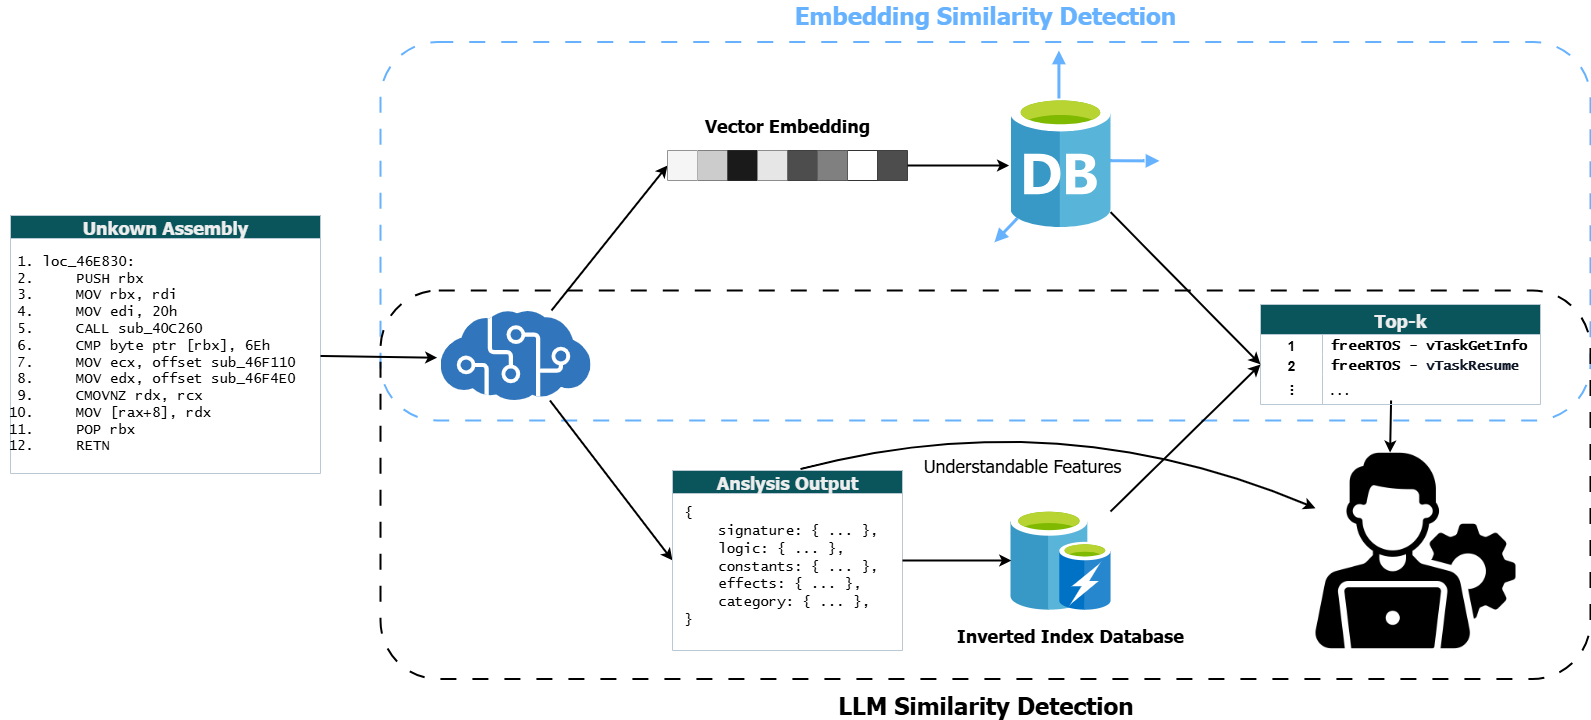
\includegraphics[width=\linewidth]{BCSD-schematic}}
\caption{Typical binary analysis workflow leveraging BCSD.}
\label{BCSD-workflow}
\end{figure}

\subsection{Problem definition}

We deem two assembly code fragments to be semantically identical if they have the same observable behavior on a system.
This type of clone is generally referred to as type four clones ~\cite{Asm2Vec,BinClone}, and is considered the most difficult
to detect. In research, it is common to use the same source code function compiled with different compilers or compilation
options to create such type four clones ~\cite{SAFE,PalmTree,OrderMatters,Asm2Vec,CLAP}.  This type of clone excludes
procedures that happen to have the same output but achieve it in different ways, for example the breadth-first search and
depth-first search algorithms. Instead of generating a binary output as to whether two code fragments are clones, the feature
vector generated for each assembly function are compared to generate a similarity score. This value is between \(0\) and \(1\) and
represents the degree of similarity between the two code fragments. This more closely aligns with real world use cases, where
two pieces of code can be highly similar but not identical. For example, two different versions of a function from the same
software deemed similar can help understand the nature of an executable, or a vulnerable function and its patched variant matched
can help assess that a vulnerability was indeed fixed. That is, the goal is to assign the highest similarity score to type four
clones, and lower similarity scores to functions that do not share semantic behavior. 

\subsection{Motivation}

BCSD is a promising technology in the field of software reverse engineering. With an ideal binary similarity engine,
the task of analyzing an unknown binary is reduced to analyzing the handful of code fragments that were genuinely developed
or modified by the software provider. All functionality coming from shared libraries or known sources, which constitutes a
large majority of modern software, would be effectively identified as such and would require no reverse engineering work.
Current technology remains far from this scenario. BCSD database maintenance is hard, because embeddings are invalidated
every model update. Current methods still exhibit a large portion of false positives, which means that human verfification
is required. Yet, these techniques give little to no insight as to why a similarity was detected between the assembly fragments.


\section{Method}

Our method is designed to address some of the pain points of state-of-the-art deep learning models for BCSD.
An important factor is that our method extracts human understandable features from an assembly function, instead
of a vector embedding. This unique advantage allows immediate human verification when a match is detected by the similarity
engine. A database of assembly functions and their interpretable features is more easily maintained, as defects can
be patched by humans, rather than having to regenerate the whole database when the model is modified.

By using any open-source or commercially available LLM, we entirely sidestep model training by leveraging the extenive
and diverse datasets that LLMs are pre-trained on.  Our method can be tuned by modifying the instructions provided to
the LLM, which is significantly simpler than having to retrain the model and regenerate embeddings for the whole database.
The underlying LLM can also replaced seamlessly without invalidating the database, meaning that our method will continue
to scale with the performance improvements of LLMs---an area which is showing impressive growth and development. Furthermore, if
a section of the prompt was edited to modify the output feature set, the database can still be maintained without
having to regenerate an output for each item. Default values or values derived from other fields in the feature set can be added,
as is standard with database migrations.

Another key advantage of our method also stems from its textual representation of the extracted feature set. As highlighted
previously, vector embeddings are computationally expensive to match against in large databases. Inverted index search is much
more scalable than nearest neighbor search, as is evident in modern search engines being able to filter through billions of documents
in a fraction of a second.

\subsection{Prompt}

The method consists of querying a large language model with a prompt crafted to extract the high-level behavioral features of
the provided assembly code fragment. The assembly code fragment does not require preprocessing. As output, the LLM generates a JSON
structure containing the extracted features. We outline the prompt made up of multiple parts, each designed to
extract specific semantic information from the assembly function. The full prompt is open-source and avaliable on Github.

\subsubsection{Framing and conditioning}

We use a prelude that contains general information about the task at hand, and the expected response.

Local LLMs, especially the smallest models, will sometimes generate nonsensical output. In our early experiments, the smallest local model
evaluated (0.5B parameters) would sometimes repeat the same line of output until it ran out of context space, or generated invalid JSON.
To combat these artifacts, we run inference again when JSON parsing fails and increase the temperature of output token
selection. This is done in a loop until valid JSON is generated. In our experiments, the maximal amount of trials required
for any query to generate valid json was three, but \(95\%\) of the generated responses from the smallest model would constitute
valid JSON without retries.

\begin{tcolorbox}[enhanced]
You are an expert assembly code analyst, specializing in high-level semantic description and feature extraction for comparative
analysis. Your goal is to analyze an assembly routine from an unspecified architecture and compiler and provide its extracted
high-level features, formatted as a JSON object. For the provided assembly routine, extract the following features and infer the
algorithm. Your output \textbf{MUST} be a JSON object conforming to the structure defined by these features.
\end{tcolorbox}

\subsubsection{Type signature}

The first feature category extracted is the type signature of the provided assembly function.
We only make the distinction between two types: Integer and Pointer. Inferring more information than these two 
primitive types has shown to be too complicated for current LLMs. We extract the number of input arguments
and their types, and also extract the return value type, if any.

\subsubsection{Logic and operations}

This section specifies what to extract from the function in terms of its logical behavior, and how to determine the kind of
operation that the assembly function performs. We list some of the operations extracted here.


\begin{itemize}
\item Indication of loops. This is determined by the presence of jump instructions that point back to a previous
instruction after some conditions have been checked.
\item Indication of jump tables. Evaluated by patterns suggesting calculated jump addresses based on
indices, or a series of conditional jumps.
\item Extensive use of indexed addressing modes.
\item Use of SIMD instructions and registers.
\item Number of distinct subroutine call targets.
\item Overall logical behavior. Possibilities include: arithmetic operations, bitwise operations, data movement and memory access,
and control flow and dispatching operations.
\end{itemize}

\subsubsection{Notable constants}

This section identifies notable integer and floating point constants.  These could be common scalar values used by
a specific cryptographic algorithm, or the signature bytes used by a file format or protocol. We exclude small
values that are used as offsets, loop counters or stack pointer adjustments.

\subsubsection{Side effects}

The prompt also monitors the side effects that the assembly function has on the system.
It reports these as a list of booleans values which state whether or not the function has
the associated side effect. Each side effect is associated with a heuristic that the language model
should use to identify them.

\begin{itemize}
    \item \textit{Modification of input arguments}. This is mainly identified when a input pointer is used as destination to a memory write.
    \item \textit{Modification of global state} is detected similarily, when writes to absolute memory addresses or addresses resolved via global
        data segment pointers occur.
    \item \textit{Memory management} is determined by the presence of calls to memory allocation and deallocation
        functions like \texttt{malloc} or \texttt{free}.
    \item \textit{Linear memory access} patterns are detected by the presence of sequential indexed memory accesses inside loops or
        across multiple successive instructions.
    \item \textit{System calls and software interrupts} are identified by the presence of the specific instructions that trigger them.
\end{itemize}

\subsubsection{Categorization}

The last section tries to assign a overall category to the assembly function, by basing it on the information
collected in the analysis. The final categorization only weakly supports the similarity search because it does
not have a large impact on the similarity score. Its purpose is to provide a concise overview for reviewers
of the analysis, who might want to understand the function or verify its similarity with the target.
Categories include: cryptographic, data processing, control flow and dispatch, initialization, error handling,
wrapper/utility, file management, etc.

\subsubsection{Examples}

To achieve the best results with our method, we utilize few-shot prompting by providing hand crafted examples along with our prompt.
In all of our evaluations, three examples are provided, and our ablation study confirms that adding more than three examples provides
little to no benefit. Providing a single example or a JSON schema in the prompt is enough to achieve good results. We do not
make use of a JSON schema because it is redundant information once examples are provided. Our examples are selected from a
diverse source of functions, and are varied in size and architecture to exemplify the space of possibilities in our evaluations.

Recent commercial LLMs have the ability to generate responses following a provided JSON schema that is aside from the input prompt
We do not make use of this capability when evaluating commercial models so that the results can be compared to local LLMs,
that do not benefit from this option.

\begin{figure}[ht]
\centering
\begin{minipage}{0.95\linewidth}
% Diff of generated output from analysis
\begin{minted}[fontsize=\small, frame=lines, framesep=2mm]{diff}
 {
   "input_parameter_count": 1,
   "input_parameter_types": [
     "Pointer"
   ],
-  "return_value_type": "None",
+  "return_value_type": "Integer",
   "dominant_operation_categories": [
     "ConditionalBranching",
     "SubroutineCall"
   ],
   "loop_indicators": false,
   "distinct_subroutine_call_targets": 2,
   "use_indexed_addressing_modes": false,
   "notable_integer_constants": [
-    "0x39"
+    "0x39",
+    "0x4"
   ],
   "notable_floating_point_constants": [],
   "count_of_distinct_immediate_values": 3,
   "modifies_input_parameters": false,
   "modifies_global_state": false,
   "memory_allocation_deallocation": false,
   "io_operations": false,
   "block_memory_operations": false,
   "number_of_interrupts_system_calls": 0,
-  "inferred_algorithm": "Undetermined"
+  "inferred_algorithm": "Initialization"
}
\end{minted}
\caption{Analysis comparison of the \texttt{sha384\_init} assembly function. Comparison between the analyses of the function compiled 
for \texttt{arm} (red) and \texttt{x86-64} (green). This pair has a similarity score of \(0.9\).}
\label{feature-diff}
\end{minipage}
\end{figure}

\subsection{Comparison}
% Artificially place table here for now
{
    \renewcommand{\arraystretch}{1.1}
    \begin{table*}[t]
    \centering
    \resizebox{\linewidth}{!}{
    \begin{tabular}{|l|c|c|l|}
    \hline
    Library       & Function count & Median function length & Description                                                          \\ \hline
    BusyBox       & 66706          & 32                     & A fairly complete unix utility set for any small or embedded system. \\
    GNU coreutils & 42545          & 31                     & The basic utilities of the GNU operating system.                     \\
    curl          & 27198          & 14                     & Command line tool to transfer data with URLs.                        \\
    ImageMagick   & 69873          & 55                     & Software suite used for editing and manipulating digital images.     \\
    OpenSSL       & 134359         & 29                     & Toolkit for general-purpose cryptography and secure communication.   \\
    PuTTY         & 12655          & 26                     & An implementation of SSH and Telnet for Windows and Unix platforms.  \\
    SQLite        & 30322          & 40                     & A small SQL database engine.                                         \\ \hline
    \end{tabular}
    }
    \caption{Dataset details.}
    \end{table*}
}

ML based methods that generate an embedding for each assembly function generally compare these vectors using numerical
methods such as cosine similarity.  Since our generated analysis is not a numerical vector but rather structured text,
we use an alternative method to compare two assembly functions. We flatten the JSON structure into a set, where each
element is the full path concatenated with the value of each element in the object. Jaccard similarity (Intesection over union)
is used to obtain a similarity score when comparing two such sets. That is, the number of identical fields in the JSON
structure is divided by the total number of elements, giving a value between \(0\) and \(1\) which we use as the similarity score.

\subsection{Dataset}

The dataset used is made of a varied set of executables, so that it represents the diversity found in real world software.
Our method is not trained, and so our dataset is only needed for evaluations. it is composed of seven open source binaries:
BusyBox ~\cite{busybox}, GNU coreutils ~\cite{coreutils}, curl ~\cite{curl}, ImageMagick ~\cite{image-magick}, OpenSSL ~\cite{openssl},
PuTTY ~\cite{putty}, and SQLite ~\cite{sqlite}. All have permissive licenses that allows their use in our evaluations. 

All binaries were compiled using \texttt{gcc} for the following architectures: \texttt{x86-64}, \texttt{arm}, \texttt{mips}, \texttt{powerpc}.
For each architecture, executables were generated for all optimization levels (\texttt{O0} to \texttt{O3}), stripped of debug symbols.
The compiled binaries were dissassembled using IDA Pro and separated into individual functions, yielding \(383,658\) assembly functions.
Functions consisting of less than three instructions were not included as part of the dataset, because of their triviality.

Pairs of equivalent functions from the same platform but distinct optimization levels are made for cross optimization
evaluation, and pairs from the same optimization level but different platforms are made for cross
platform evaluation. For example, the \texttt{MD5Init} functions in \autoref{asm-diff} compiled with \texttt{-O0} (left) and
\texttt{-O3} (right) for \texttt{x86-64} form a pair for cross optimization retrieval, whereas functions compiled with \texttt{-O0}
for \texttt{x86-64} (left) and \texttt{mips} (center) form a pair for cross architecture retrieval.

\section{Experiments}

Our experiments are run on a virtual machine with 8 Intel Xeon Gold 5218 cpu cores, \(100\) GB of RAM, and two NVIDIA Quadro RTX
6000 GPUs each having  \(24\) GB of RAM. First, we select the LLM best suited for our subsequent experiments. Second, we compare our
method against other state-of-the-art ML based approaches to BCSD on our dataset. Third, we perform ablation studies on our method,
to determine how the size of the model, the number of examples provided, and the different sections of the prompt contribute to our results.
Finally, we demonstrate that the features extracted from our novel method are not properly represented in state-of-the-art embedding methods,
and that by combining our method with an embedding model yields significantly better results that state of the art approaches.

\subsection{Evaluation method}

The mean reciprocal rank (MRR) and first position recall (Recall@1) metrics are used for evaluation and comparison to other methods
~\cite{deprio,code-not-lang,Asm2Vec,CLAP,SAFE}.
A pool of assembly function pairs is used for evaluation, where both assembly fragments in a pair come from the same source function.
For each pair, we compare the generated features for the first element of the pair with all second elements of the pairs contained
in the pool.  For example, consider a pool of ten pairs \((a_i, b_i)\) for \(i \in [1, 10]\), where \(a_i\) is compiled for the \texttt{arm}
architecture with optimization level \(3\), and \(b_i\) is compiled for the \texttt{mips} architecture with the same optimization
level. The features generated for function \(a_1\) is compared for similarity with the features of \(b_i\) for \(i \in [1, 10]\).
A ranking is generated by ordering these comparisons from most to least similar. Recall@1 is successful
if \(b_1\) is found to be the most similar function, and the reciprocal rank metric is calculated with \autoref{mrr}.
\begin{equation} \label{mrr}
\frac{1}{\text{rank}(b_1)}
\end{equation}
\noindent The Recall@1 metric is calculated by dividing the number of successful recalls by the total number of pairs, and the
MRR metric is calculated by averaging the reciprocal rank of each pair.

\subsection{LLM Selection}

Before evaluating our method against the baselines, we compare different LLMs available to select our backbone for the remaining experiments.
For the local model, three options are considered: Qwen2.5 Coder ~\cite{qwen2} with sizes \(0.5\)B, \(1.5\)B, \(3\)B, and \(7\)B;
Gemma 3 ~\cite{gemma3} with sizes \(1\)B and \(4\)B; and  Qwen3 \(4\)B ~\cite{qwen3}. We preselected these models because they are open source,
small enough to fit in most modern GPUs when quantized, and small enough to fit within our GPU with
\(24\) GB of VRAM unquantized. We did not consider mixture-of-experts models because they are much larger, and the specificity of our
workload is likely to result in only a subset of expert being heavily used. We selected a small set of tasks that are representative
of the extensive experiments conducted against the baselines. There are two cross optimization evaluations, and one cross architecture 
evaluation.
{
    \renewcommand{\arraystretch}{1.1}
    \begin{table}[h]
    \centering
    \begin{tabular}{|l|ccc|} \hline
    Model            & \tt O0--O3 & \tt O2--O3 & \tt arm--x86-64 \\ \hline
    Qwen2.5 Coder 7B & 0.558      & 0.725      & 0.498            \\
    Qwen3 4B         & 0.550      & \bf 0.850  & 0.564            \\
    Gemma 3 4B       & \bf 0.571  & 0.839      & \bf 0.594        \\ \hline
    \end{tabular}
    \caption{Results of the selected evalutations for local model selection, using a pool size of \(100\).}
    \end{table}
}

In all experiments on local models, the input context size is limited to \(4096\) tokens, and the maximum output tokens to generate is set to \(512\).
Very large assembly functions that do not fit within the input tokens are truncated. The more recent Qwen3 and Gemma 3
models perform better for their size than Qwen2.5. They match or surpass Qwen2.5 Coder in most metrics while being around \(40\%\)
smaller. However, we selected Qwen2.5 Coder for the remaining experiments because it provides many small sizes for our ablation study,
and is more stable than these new models.

For the commercial model, we preselected GPT 4.1 Mini \cite{gpt4} and Gemini 2.5 Flash \cite{gemini2.5}.
These were chosen mainly because of their low cost and availability. The same subset of evaluations as for local models is performed to determine
the model to use for the remaining evaluations.
{
    \renewcommand{\arraystretch}{1.1}
    \begin{table}[h]
    \centering
    \begin{tabular}{|l|ccc|} \hline
    Model            & \tt O0--O3 & \tt O2--O3 & \tt arm--x86-64 \\ \hline
    Gemini 2.5 Flash & \bf 0.674  & \bf 0.865  & \bf 0.766        \\
    GPT 4.1 Mini     & 0.662      & 0.811      & 0.755            \\ \hline
    \end{tabular}
    \caption{Results of the selected evalutations for commercial model selection, using a pool size of \(100\).}
    \end{table}
}

To provide a similar environment to local models, functions are truncated to a maximum length of \(128\) instructions.
We selected Gemini 2.5 Flash because it performs best and offers a better infrastructure. Compared to GPT 4.1 Mini's \(10\) seconds
latency per request, Gemini is almost able to handle a request every second, making it easier to iterate on our evaluations.

\subsection{Clone search with different optimization levels}

{
    \renewcommand{\arraystretch}{1.3}
    \begin{table*}[t]
    \centering
    \resizebox{\linewidth}{!}{
    \begin{tabular}{l|cccccc|cccccc}
    \Xhline{2\arrayrulewidth}
    \multirow{2}{*}{Model} & \multicolumn{6}{c|}{MRR}                                  & \multicolumn{6}{c}{Recall @ 1}                                                        \\ \cline{2-13}
                           & \tt O0--O1 & \tt O0--O2 & \tt O0--O3 & \tt O1--O3 & \tt O2--O3 & average     & \tt O0--O1 & \tt O0--O2 & \tt O0--O3 & \tt O1--O3 & \tt O2--O3 & average   \\ \hline
    Order Matters          & 0.006      & 0.008      & 0.006      & 0.006      & 0.006      & 0.006       & 0.001      & 0.002      & 0.001      & 0.000      & 0.001      & 0.001     \\
    SAFE                   & 0.189      & 0.200      & 0.189      & 0.218      & 0.171      & 0.193       & 0.000      & 0.063      & 0.063      & 0.063      & 0.000      & 0.038     \\
    PalmTree               & 0.020      & 0.019      & 0.230      & 0.314      & \bf 0.878  & 0.292       & 0.006      & 0.007      & 0.080      & 0.184      & 0.676      & 0.191     \\
    Asm2Vec                & 0.494      & 0.460      & 0.444      & 0.535      & 0.563      & 0.499       & 0.290      & 0.252      & 0.234      & 0.343      & 0.376      & 0.299     \\
    CLAP                   & 0.244      & 0.221      & 0.214      & 0.550      & 0.781      & 0.402       & 0.187      & 0.176      & 0.168      & 0.455      & 0.707      & 0.339     \\ \hline
    Qweni 2.5 7B           & 0.471      & 0.412      & 0.343      & 0.456      & 0.608      & 0.458       & 0.342      & 0.301      & 0.234      & 0.345      & 0.488      & 0.342     \\
    Gemini 2.5 Flash       & \bf 0.739  & \bf 0.672  & \bf 0.568  & \bf 0.700  & 0.816      & \bf 0.699   & \bf 0.646  & \bf 0.579  & \bf 0.485  & \bf 0.618  & \bf 0.758  & \bf 0.617 \\ \Xhline{2\arrayrulewidth}
    \end{tabular}
    }
    \caption{Evaluation of the baselines and our method on cross optimization retrieval with a pool size of \(1000\).
    All functions are compiled for the \texttt{arm} architecture using gcc with the optimization levels specified for each column.
    Three examples are provided with our prompt.}
    \label{x-opt}
    \end{table*}
}

This experiment benchmarks the capability of the baselines and our method for detection of similar code fragments across
different optimization levels. We first present the baselines and then show our results.

\noindent \textbf{Baselines.} Order Matters ~\cite{OrderMatters} combines a BERT language reprensentation
model ~\cite{BERT} along with two control flow graph embedding models
to perform BCSD. It uses BERT to learn the embeddings of instructions and basic blocks from the function,
passes the CFG through a graph neural network to obtain a graph semantics embedding, and sends the adjacency
matrix of the CFG through a convolutional neural network to compute a graph order embedding. These embeddings
are then combined using a multi-layer perceptron, obtaining the assembly function's embedding. This method
supports cross architecture and cross platform tasks, although its implementation is only trained on \texttt{x86-64}
and \texttt{arm} for cross architecture retrieval.

SAFE ~\cite{SAFE} first encodes each instruction of an assembly function into a vector,
using the word2vec model ~\cite{word2vec}. Using a Self-Attentive Neural Network ~\cite{SANN}, SAFE then converts the sequence of instruction
vectors from the assembly function into a single vector embedding for the function. Like all other baslines, SAFE requires
pre-training, and can perform cross architecture similarity detection. However, it was only trained on the \texttt{AMD64}
and \texttt{arm} architectures.

Asm2Vec ~\cite{Asm2Vec} inspired the SAFE model. It is one of the first methods to use a NLP based approach to tackle
the BCSD problem. It interprets an assembly function as a set of instruction sequences, where each instruction sequence
is a possible execution path of the function. It samples these sequences by randomly traversing the CFG of the assembly
function, and then uses a technique based on the PV-DM architecture ~\cite{PV-DM} (an extension of word2vec that embeds entire documents)
to generate an embedding for the assembly function.

A more recent BCSD model, PalmTree ~\cite{PalmTree}, also bases its work on the BERT model ~\cite{BERT}.
It considers each instruction as a sentence, and decomposes it into basic tokens. The model is trained
on three tasks. (1) As is common for BERT models, PalmTree is trained on masked language modeling. (2)
It is also trained on context window prediction, that is, predicting whether two instructions are found
in the same context window of an assembly function. (3) Finally, the model is trained on def-use prediction---predicting
whether there is a definition-usage relation between two instructions. This method supports
both cross architecture and cross optimization tasks, although its reference implementation is only
trained on cross compiler similarity detection.

The model CLAP ~\cite{CLAP} uses the RoBERTa ~\cite{RoBERTa} base model to perform assembly function embedding.
It is adapted for assembly instruction tokenization, and directly generates an embedding for
a whole assembly function. It is also comes with a text embedding model, CLAP-text, so that classification can
be performed using human readable classes. Categories or labels are embedded with the text model, and the
assembly function with the assembly embedding model. The generated embeddings can be compared with cosine similarity to
calculate whether the assembly function is closely related or opposed to the embedded category. This model was only trained
for the \texttt{x86-64} architecture compiled with \texttt{gcc}, although it supports other architectures and could be trained on
them.

We present the results of our method evaluated on both the local model, Qwen2.5-Coder 7B Parameters, and the commercially deployed model,
Gemini 2.5 Flash. As evident in \autoref{x-opt}, the hardest retrieval task is between optimization levels \(0\) and \(3\),
highlighting the substantial difference between unoptimized and maximally optimized code (see \autoref{asm-diff}).
At optimization level \(0\), functions perform a lot of unessecary actions, such as extensively moving
data between registers and perform conditional evaluation of expressions that return a constant value. The generated code
is mostly left untouched by the optimizer. At optimization level \(3\), the compiler will inline simple functions into the
body of the caller, meaning that jumps and calls to other places in the binary are replaced by the destination's instructions.
Some loops are unrolled, so that each iteration of the loop is laid out sequentially instead of performing a conditional check
and a jump to the loop's initial instruction. Also, instructions can be heavily reordered to achieve best performance for the targeted
hardware, while keeping the observable behavior of the program untouched.

The baselines mostly perform worse than expected on this evaluation. As our own dataset is used
rather than the one each baseline is pre-trained on, overfitting in the training process may be the cause of this poor performance,
as also observed by Marcelli et al. \cite{cisco}. Compared to the baselines, one of our method's advantage is that it requires no
specific training other than the pre-traning process performed by open source model developers. It readily acheives good results,
meaning our method generalizes well to unseen settings.

\subsection{Clone search with different architectures}

{
    \renewcommand{\arraystretch}{1.3}
    \begin{table*}[!t]
    \centering
    \resizebox{\linewidth}{!}{
    \begin{tabular}{l|cccc|cccc}
    \Xhline{2\arrayrulewidth}
    \multirow{2}{*}{Model} & \multicolumn{4}{c|}{MRR}                                 & \multicolumn{4}{c}{Recall @ 1}                           \\ \cline{2-9}
                           & \tt arm--x86-64 & \tt powerpc--x86-64 & \tt mips--x86-64 & average   & \tt arm--x86-64 & \tt powerpc--x86-64 & \tt mips--x86-64 & average   \\ \hline
    Order Matters          & 0.007           & 0.007               & 0.007            & 0.007     & 0.002           & 0.000               & 0.001            & 0.001     \\
    SAFE                   & 0.239           & 0.187               & 0.196            & 0.207     & 0.063           & 0.063               & 0.063            & 0.063     \\
    PalmTree               & 0.037           & 0.036               & 0.018            & 0.030     & 0.031           & 0.013               & 0.007            & 0.017     \\
    Asm2Vec                & 0.242           & 0.293               & 0.417            & 0.317     & 0.085           & 0.113               & 0.231            & 0.143     \\
    CLAP                   & 0.416           & \bf 0.523           & 0.494            & 0.478     & 0.334           & \bf 0.443           & 0.415            & 0.397     \\ \hline
    Qwen 2.5 7B            & 0.263           & 0.201               & 0.202            & 0.222     & 0.165           & 0.108               & 0.110            & 0.128     \\
    Gemini 2.5 Flash       & \bf 0.548       & 0.520               & \bf 0.525        & \bf 0.531 & \bf 0.436       & 0.414               & \bf 0.417        & \bf 0.422 \\ \Xhline{2\arrayrulewidth}
    \end{tabular}
    }
    \caption{Evaluation of the baselines and our method on cross architecture retrieval with a pool size of \(1000\).
    All functions are compiled with optimization level \(2\) using \texttt{gcc} for the architectures specified in each column.
    Three examples are provided with our prompt.}
    \label{x-arch}
    \end{table*}
}

Different CPU architectures have varying assembly code languages. It is hard for BCSD methods that analyze assembly code to support
multiple architectures. These methods need to accurately represent two functions with completely different syntaxes but with identical
semantics as being very similar in terms of their feature vector or embedding. Hence, methods that use CFG analysis have a better chance
at supporting many architectures, since the structure of the CFG itself is architecture agnostic. However, the basic blocks that constitute
this graph are still in assembly code, which does not fully resolve the issue. Furthermore, there exists many different variants of each
instruction set, because each new version of an architecture brings new instructions to understand and support. With deep learning methods,
this requires training or fine-tuning the model to understand a new language variant every time. Afterwards, all embeddings in a BCSD database need to
be regenerated. Our method does not directly address this issue, but brings a significant improvement. It indirectly makes use of the vast
amount of data used to train foundational LLMs. Since a LLM has extensively seen all of the mainstream CPU architectures and their dialects
in its training data, it is able to grasp their meaning and extract features from them. Also, if the model in use seems to poorly comprehend a
specific architecture, it can be replaced with one that better performs the specific platform without invalidating the BCSD database.

Our method surpasses the baselines, but more work in this area is clearly still required. The recall@1 metrics show that the our method
is able to rank the the correct assembly fragment in first place only \(42\%\) of the time on average.

\subsection{Ablation on model size}

\begin{figure}[htbp]
\centerline{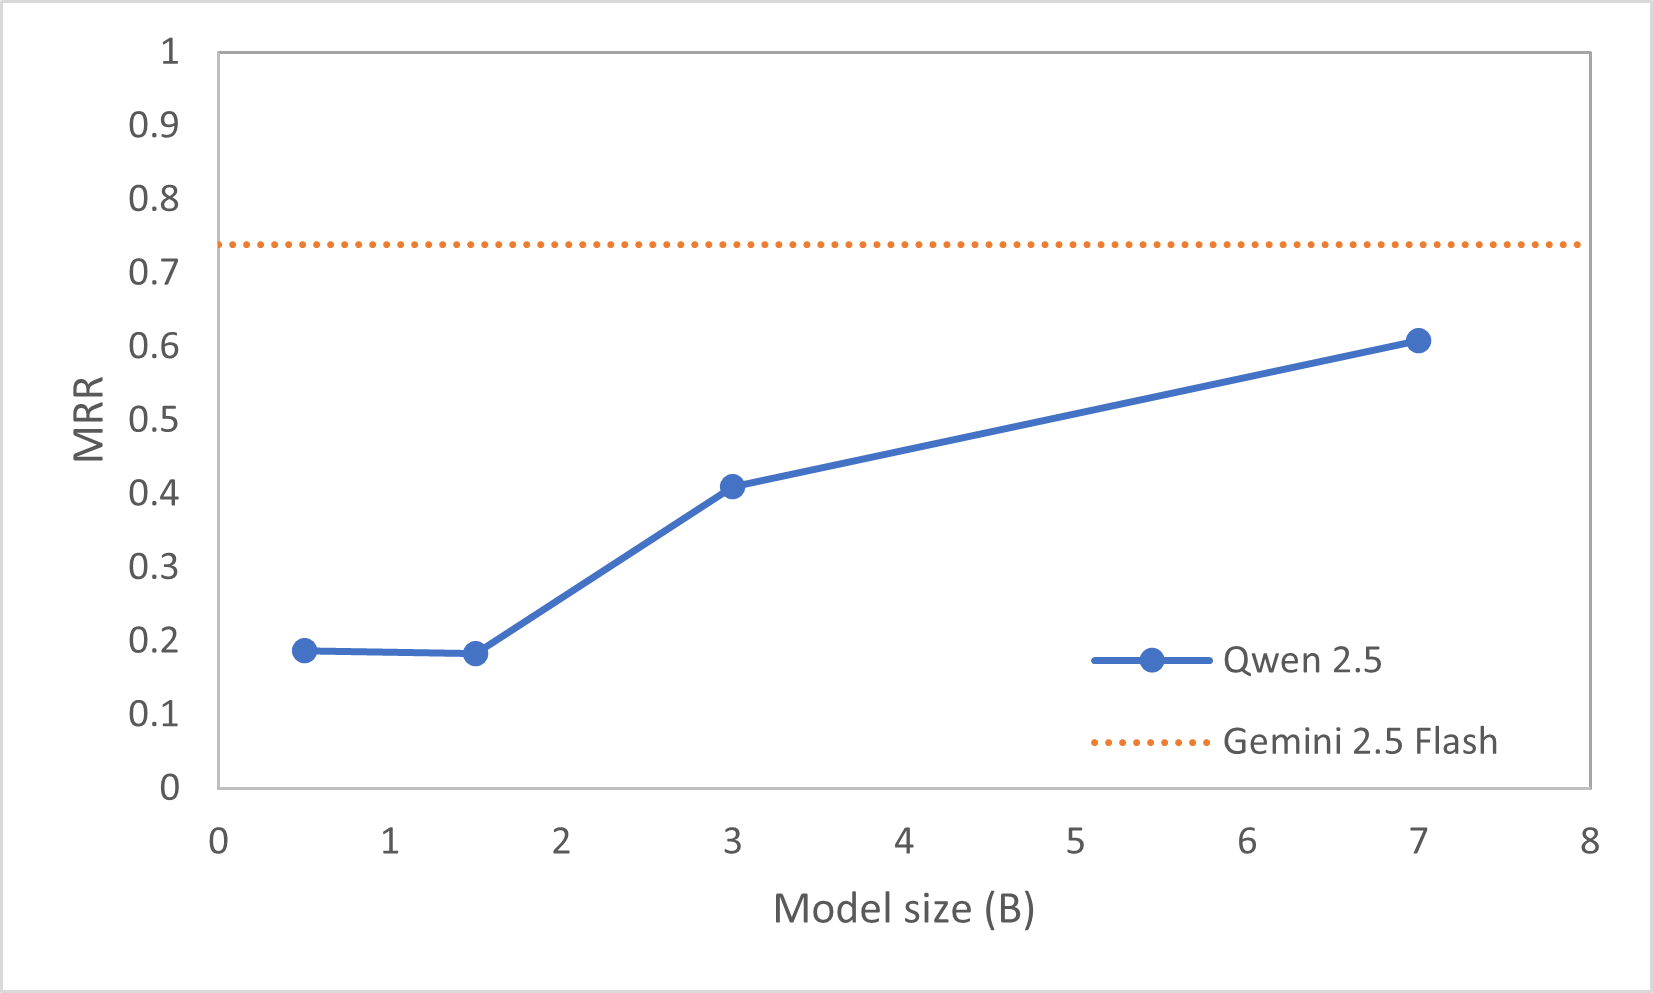
\includegraphics[width=\linewidth]{size-ablation}}
\caption{MRR performance for cross optimization retrieval against the number of parameters in the LLM. All assembly functions are compiled
with \texttt{gcc} for the \texttt{arm} architecture. Retrieval is performed between optimization levels \(0\) and \(1\) with a pool of \(1000\) assembly functions.
Three examples are provided with our prompt.}
\label{size-abl}
\end{figure}

In this experiment, we vary the LLM size to determine the correlation between the number of parameters in the LLM and the performance
of our method on BCSD retrieval. Our results generally follow the scaling laws for neural language models ~\cite{scaling-laws}, in that increasing
the model size does significantly improve the results generated.

From our observations, LLMs with less than \(3\)B parameters do not seem to comprehend the analysis task when
they are not provided with any examples. When provided with examples, these small models will mimic the examples provided without basing the
output on the assembly function in the query. We can clearly see a form of sub-linear increase in performance with respect to model size.
The Gemini 2.5 Flash model architecture is not disclosed at the time of writing, but we can expect the model to have an order
of magnitude more parameters, than our local models, and may use a mixture of expert architecture, based on disclosed previous Gemini model versions.

\subsection{Ablation on examples}

\begin{figure}[]
\centerline{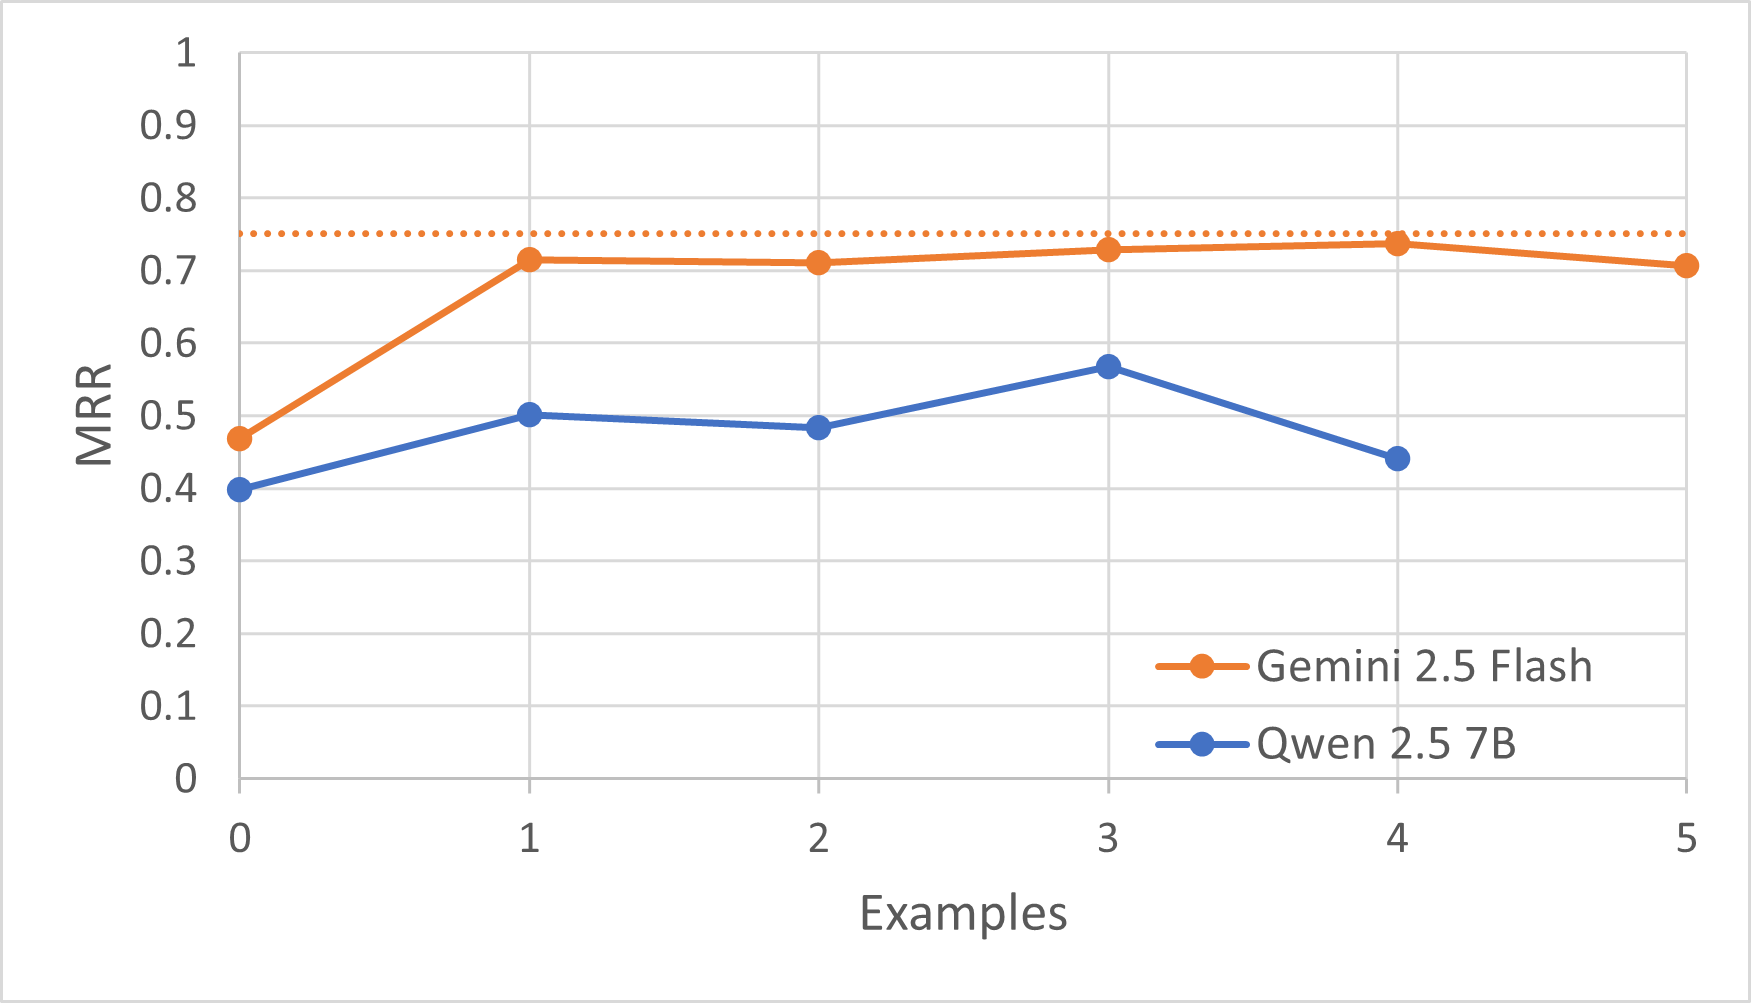
\includegraphics[width=\linewidth]{examples-ablation}}
\caption{MRR performance for cross optimization retrieval against the number of examples provided in the prompt. Functions are compiled
using gcc for the \texttt{x86-64} architecture. A pool of \(100\) assembly functions is used, with retrieval between optimization levels \(0\) and \(3\)
for Gemini 2.5 Flash, and \(0\) and \(1\) for Qwen 2.5 \(7\)B.}
\label{ex-abl}
\end{figure}

By providing hand crafted examples to the large language model, we are able to increase the performance of the assembly function analysis.
This follows the general observations behind few show prompting ~\cite{few-shot}. Providing a single example significantly increases the retrieval
scores, but providing more than one provides very limited increases in scores. Interestingly, a smaller model such as Qwen 2.5 \(7\)B still sees
marginal increase in MRR scores as the number of examples increases up to three. This relates to our previous observation
that small LLMs rely more on the provided examples than larger models. Another evidence of this is the number of invalid JSON outputs generated by
Qwen 2.5 \(7\)B. When no examples are provided, approximately \(3\%\) of queries generate an invalid output. With only one example, no invalid
outputs are generated, and the same applies when two or three examples are provided.

Another interesting result is the fact that when providing enough examples, the system prompt has very little impact on the retrieval scores.
This is depicted by the green data points in \autoref{ex-abl}, where only examples are provided with an empty string as the system prompt.
This suggests that the examples themselves contain enough information for the model to perform the analysis, without being expained 
exactly how.

With our experimental configuration, providing four examples to Qwen 2.5 \(7\)B significantly decreases its MRR scores. That is because
the examples almost completely use the full context window that we provide to the LLM. As such, most query assembly functions are
too large and thus truncated, which loses information about our query.

The dotted line in \autoref{ex-abl} represents the MRR score obtained by providing no examples to Gemini 2.5 Flash, but providing a reference JSON
schema for the model to follow. The scores being equivalent shows that Gemini does not base itself on the provided examples, but only
uses them to understand the JSON schema required. In all our other evaluations, we provide examples instead of a JSON schema because local
models do not have the capability of generating output based on a schema built-in.

\subsection{Ablation on the prompt used}

\begin{figure}[htbp]
\centerline{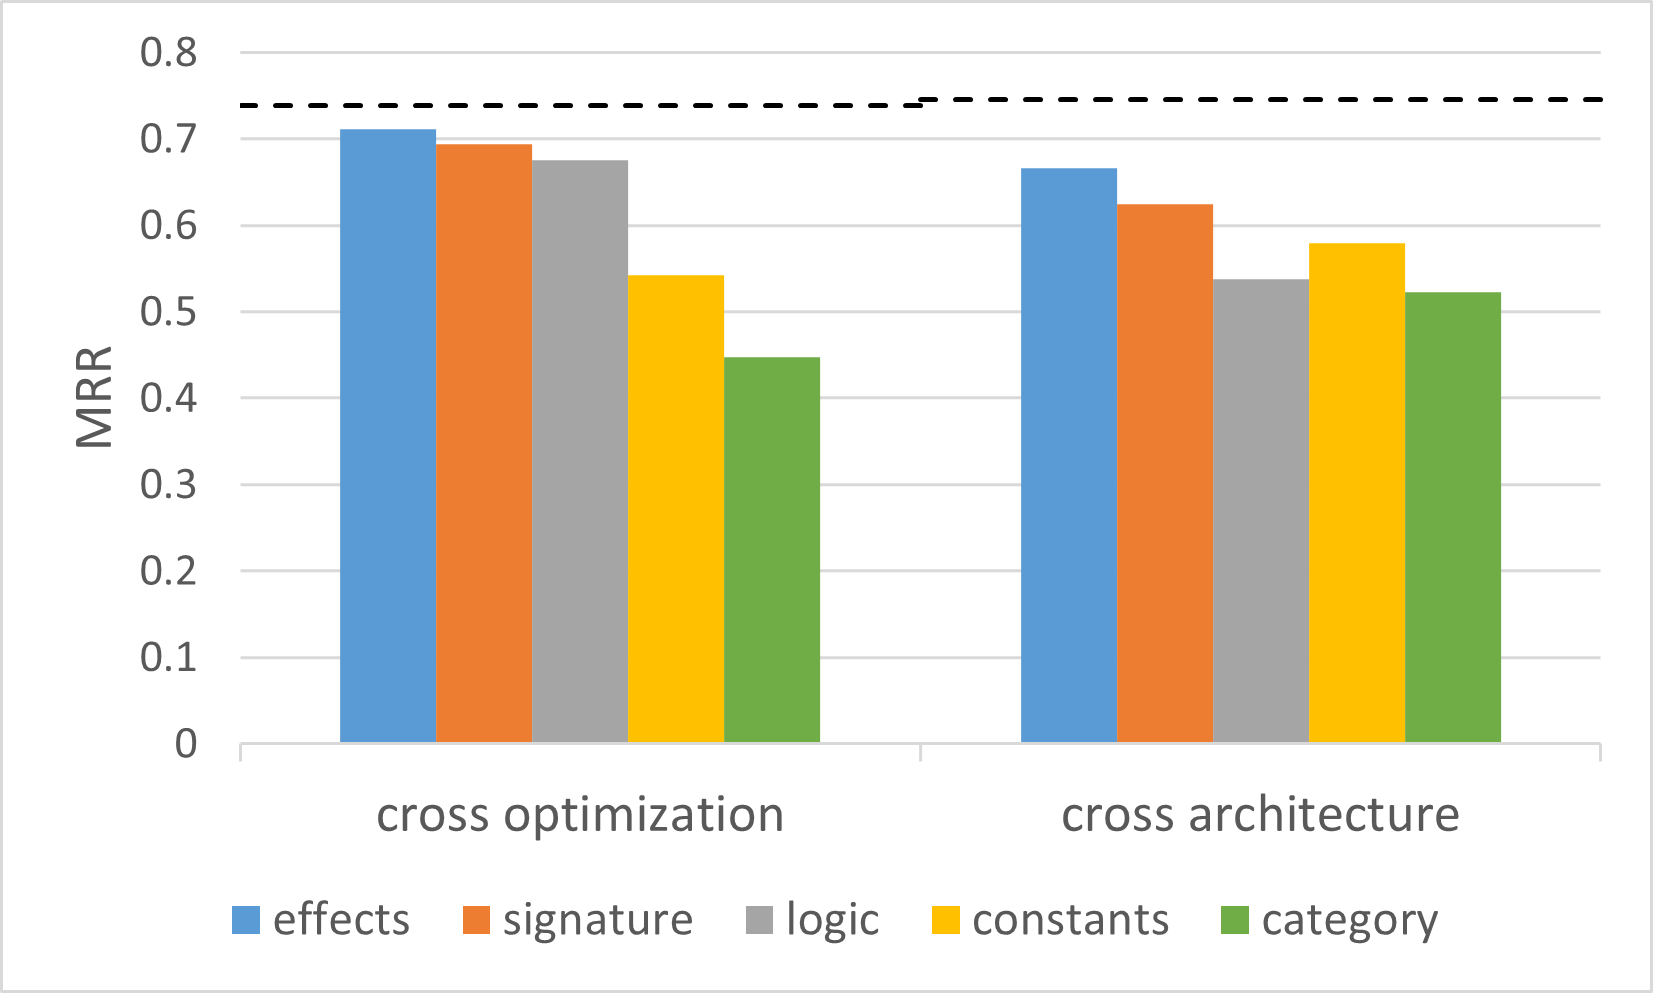
\includegraphics[width=\linewidth]{prompt-ablation}}
\caption{
MRR performance with one section removed from the prompt. Cross optimization retrieval is done between fragments at
optimization levels \(0\) and \(3\), with all functions compiled for the \texttt{x86-64} architecture. Cross architecture retrieval is done between functions
compiled for \texttt{arm} and \texttt{x86-64}, all compiled using optimization level \(2\). Both tasks are done with a pool size of \(100\). The dotted lines
show the MRR score for the prompt without any sections removed. A smaller bar means the prompt section has more impact on the results.}
\label{prompt-abl}
\end{figure}

To verify that each section of our prompt brings meaningful insight into the assembly function analysis task, we perform an ablation
study by removing one section of the prompt while keeping others intact. We notice that all individual sections bring a positive
outcome to the overall results, but some sections of the prompt have a larger impact than others. In particular, the categorization and
notable constants sections have the most impacts on cross optimization retrieval. The categorization section causes an increase of almost
\(0.30\) on the MRR metric, when evaluated on the the hardest cross optimization task. The notable constants sections brings an increase of
almost \(0.20\) on the MRR for the same task. This result is justified by the comparatively large range of accepted values for both features.
For example, the list of notable constants has many more possible values and thus has more variability in the output compared to a set
of booleans, such as those in the side effects prompt section.

The story is slightly different when this ablation study is performed for cross architecture retrieval. As seen on \autoref{prompt-abl},
there is a smaller difference between the least and most influential prompt sections. The categorization and notable constants sections
are significantly less impactful than they were for the cross optimization study, while the other three sections have a larger impact.
For instance, the categorization section went from having an impact of \(0.30\) on the MRR to having an impact \(0.22\), while the logic
section is more influential, going from \(0.06\) to \(0.20\) in MRR impact.

\subsection{Combined Method}

Our method has shown to be an excellent generalist on BCSD retrieval tasks. Nevertheless, models trained for assembly function understanding
and BCSD remain benefitial in specific subdomains, such as supporting niche architectures or understanding similarity through
specific obfuscation methods. The state-of-the-art embedding models are much smaller than our method in terms of parameter count.
For instance, the CLAP ~\cite{CLAP} model baseline is only \(110\)M parameters, compared to the billions required to perform our method.
Their small size potentially allows for CPU execution on small workloads. The cost of training such models is still very expensive,
but once trained, they are much faster than LLM inference.

To achieve the best of both worlds, we experiment with combining the similarity scores from an embedding model and our prompting method.
Our evaluation method consists of generating both an embedding and a LLM analysis for each function. The embedding similarity \(s_e\) is calculated
using cosine similarity, and the analysis similiarity \(s_a\) is calculated using jaccard similarity. Both similarity scores are then combined
with equal weight.
\[
    S = \frac{s_e + s_a}{2}
\]

In a real life scenario, combining both methods could be performed by using our textual representation as a pre-filter, and then calculating
the embedding representation. As such, the scalability and maintainability of the underlying BCSD database is maintained, while allowing a flexible
choice of embedding based BCSD model. That is, an inverted index database is maintained for the pre-filter query. Once this query is completed, the
top-\(k\) results can be refined using an embedding model, by calculating the embeddings only for those \(k\) candidates. With this approach,
the decision to use an embedding model, and which one to use, can be made dynamically.

To provide a method that keeps all of the advantages of our presented work, we use Qwen3-Embedding \(4\)B as the embedding model for this experiment.
As such, the combination still does not require any training nor fine-tuning. As shown in \autoref{composite}, off-the-shelf embedding models
based on a LLM perform very well. Furthermore, using a generic embedding model means that it can inexpensively be replaced by a new generation
(the training phase is performed by the open source model developers).

{
\renewcommand{\arraystretch}{1.1}
\begin{table*}[tb]
\centering
\begin{tabular}{l|c|c|c}
\Xhline{2\arrayrulewidth}
                       & Gemini 2.5 Flash & Qwen Embedding & Combined  \\ \hline
\tt O0 -- O1           & 0.646            & 0.640          & \bf 0.910 \\
\tt O0 -- O2           & 0.579            & 0.554          & \bf 0.843 \\
\tt O0 -- O3           & 0.485            & 0.518          & \bf 0.759 \\
\tt O1 -- O3           & 0.618            & 0.640          & \bf 0.855 \\
\tt O2 -- O3           & 0.758            & 0.783          & \bf 0.921 \\
\tt arm -- x86-64      & 0.436            & 0.334          & \bf 0.736 \\
\tt powerpc -- x86-64  & 0.414            & 0.443          & \bf 0.746 \\
\tt mips -- x86-64     & 0.417            & 0.415          & \bf 0.729 \\ \Xhline{2\arrayrulewidth}
\end{tabular}
\caption{Comparison between Qwen3-Embedding 4B, Gemini 2.5 Flash, and the combination of both. The retrieval task is performed on both cross
optimization and cross architecture settings. For cross optimization, the binaries are compiled for the \texttt{arm} architecture, for cross architecture,
the binaries are compiled with optimization level \(2\). A pool of 1000 assembly functions is used throughout. Only Recall@1 scores are presented.}
\label{composite}
\end{table*}
}

The combined method significantly surpasses both the embedding and analysis methods alone. Seen differently, the embedding and analysis supplement
each other, meaning that our analysis extracts features from the assembly function that are not properly represented in the embedding model.

\section{Related Work}
\label{related-work}

\subsection{Early BCSD methods}

\textbf{Static analysis.} Traditional methods make use of static analysis to detect clone assembly routines. With these methods, a trade-off has
to be made between the robustness to obfuscation and architecture differences, and the performance of the algorithm. ~\cite{BCSDsurvey}
Control flow graph analysis and comparison ~\cite{BinDiff,graph-bug-search} is known to be robust to syntactic differences, but often
involves computationally intractable problems. Other algorithms that use heuristics such as instruction frequency,
longest-common-subsequence, or locality sensitive hashes ~\cite{clones.net,op-seq,sem-hash} are less time consuming, but tend to fixate on the syntactic
elements and their ordering rather than the semantics.

\textbf{Dynamic analysis.} This method family consists of analyzing the features of a binary or code fragment by monitoring its runtime behavior.
This method is compute intensive and requires a cross-platform emulator, but completely sidesteps the syntactic aspects of binary code
and solely analyzes its semantics. ~\cite{BCSD} As such, this method is highly resilient to obfuscations, but requires a sandboxed environment
and is hard to generalize across architectures and application binary interfaces ~\cite{blanket-exec}.

\subsection{LLM based software analysis}

Researchers have found many related applications of Large language models to binary and software analysis.
For vulnerability detection, FuncVul ~\cite{funcVul} is a GraphCodeBERT model fine-tuned to detect whether a provided
source function is vulnerable. The dataset generation process makes use of a LLM to rewrite each function in a generic maner,
erasing variable and function names. The LLM is also used in their method to predict the lines on which the vulnerability is found.
LLM4Decompile ~\cite{llm4decompile} tries to utilise LLMs for decompilation. An open source LLM is fine-tuned to learn the source code
representation of an assembly function. Fang et al. ~\cite{source-analysis} measure the competency of LLMs for source code analysis,
with a focus on obfuscated source code. Their results match our findings, that LLMs are efficient at code analysis, except in cases
of advanced obfuscation techniques. LLM based fuzzing is another area that has recently gained interest. For instance,
Asmita et al. ~\cite{llm-fuzz} use a LLM to generate the initial seed of a fuzzing pipeline on the BusyBox ~\cite{busybox} executable.

\section{Conclusion}

Our method for BCSD introduces a shift in perspective compared to previous state-of-the-art BCSD embedding models. However,
this new approach maintains some of the known limitations and also brings new limitations. Most importantly, this
method makes use of massive models compared to previous methods. A powerful set of GPUs is required when generating
feature sets for a large pool or database. This favors centralised databases with large amounts of assembly fragments over
locally maintained databases with hundreds or thousands of functions. Otherwise, a commercially deployed LLM can be used at a
cost, but concerns surrounding data privacy can legitimately be raised. Another potential limitation is the size of the feature
set extracted during assembly analysis. As shown, our prompt performs very well with pool sizes of \(1000\) assembly functions,
however, this may not be the case when comparing millions of feature sets, as is the case in production databases.

We remain confident that our method brings significant improvements to the current landscape of BCSD, by resolving
many of the previously acknowledged limitations. Our method does not require any form of training, and can be performed with any LLM
available. It also offers a distinct advantage over the current state-of-the-art, because the feature vectors generated are human
interpretable. This makes the method easily tunable by human experts. The similarity scores are much more easily verifiable, and
cases of incorrect similarity detection can be explained using the generated feature set. Furthermore, this method can be scaled to
databases containing millions of assembly functions compared to embedding models, since inverted index search has a lower time
complexity than nearest neighbor search, and remains accurate compared to approximated nearest neighbor search methods.

\subsection{Future research}

Our results open avenues for further investigation in LLM based BCSD, and more broadly in LLM assisted reverse engineering.
A few of these oportunities are outlined here.

\subsubsection{Reasoning models}

State-of-the-art LLMs are fine tuned to natively use chain of thought methods ~\cite{c-o-t} before answering the query.
These models are known as reasoning models, and it has been shown that this method of inference produces more accurate and
higher quality responses ~\cite{c-o-t,reasoning,thinking-llm}. It may be worth evaluating whether this style of model performs better than
non reasoning models (as used in our research) on assembly function analysis.

\subsubsection{Fine-tuning}

As stated, our method does not require fine-tuning, and was not evaluated on fine-tuned performance. Developing a fine-tuning step
for assembly code understanding and analysis may prove to be efficient and bring significant improvements to our method.
An example of such technique would be distillation ~\cite{distillation}. With distillation, a large model is used to train or fine-tune a
much smaller model. For example in our experiments, Gemini 2.5 Flash could have been used to fine tune the small Qwen2.5-Coder models.
Since there is no ground truth in text generation, the distillation process uses the large model's output as ground truth
to train the smaller model. As we have shown, a large model such as Gemini 2.5 Flash performs remarkably better than a
small model such as Qwen2.5 7B at assembly understanding. We believe the distillation process could considerably reduce this gap.

\subsubsection{Output Format}

Our method uses the JSON output format so that the output generated is comparable with others and a similarity metrics can be deduced.
This format was chosen because it is ubiquitous and its syntax is straightforward to produce for LLMs, and easily understandable for humans.
However, finding the best trade-off between output interpretability, compute requirements, and similarity detection capabilities remains
an open problem. One possibility is to loosen the restrictions on the output format and use a sentence similarity method to determine
the similarity between function analyses. On the contrary, another possibility is to use the analysis cabapilities at a smaller scale,
for example analyzing single basic blocks and combining these analyses into a more comprehensive structure for a whole assembly function.
In any case, more experimentation is required to find optimal balance.

\subsubsection{Other integrations}

Our work proves the competency of LLMs in understanding and analyzing assembly code. From this point, different approaches
to incorporating LLMs into assembly analysis workflows can be considered. First, instead of using LLMs for feature extraction,
they could be used to explain the similarity between two functions, once this similarity has been determined using an unexplainable
method such as embeddings. Furthermore, it could be used as a decision maker as to whether the two code fragments are similar enough
to be considered clones. Often times, the assembly function used as query is not even part of the BCSD database. The remarkable versatility
of LLMs underscores the need for further research to determine where they can effectively support the reverse engineering workflow and where
their utility remains limited.

%-------------------------------------------------------------------------------
\section*{Acknowledgments}
%-------------------------------------------------------------------------------

The USENIX latex style is old and very tired, which is why
there's no \textbackslash{}acks command for you to use when
acknowledging. Sorry.

\textbf{Do not include any acknowledgements in your submission which may deanonymize you (e.g., because of specific affiliations or grants you acknowledge)}

%-------------------------------------------------------------------------------
% optional clearing of the page
\cleardoublepage
\appendix
\section*{Ethical Considerations}
\textbf{Within up to one page, explain the ethical considerations of your work. This appendix must have exactly this title, otherwise you will risk desk rejection. Carefully study the Ethics Guidelines before submitting your paper.}

Stakeholders:

The direct stakeholders in this research's outcomes include:
\begin{itemize}
\item Users of reverse engineering software and BCSD tools.
\item Software developers trying to prevent their software from being reconstructed.
\item LLM providers and developers.
\end{itemize}

We believe that our method risks having postive outcomes for reverse engineering software users and
the LLM industry, but risks having a negative impact on developers trying to hinder reverse engineering of their binaries. As
thouroughly discussed in this research, we believe our method improves BCSD on many aspects. This benefits users of such tools,
and also benefits LLM providers and developers, because our work presents yet another use of their technology, and thus risks
increasing its usage. An increase in usage is positive for developers of open source models, and LLM providers may also gain more users
which is a positive consequence. It may become harder for software developers to prevent reverse engineering of their software.

Software providers and users are also risk being impacted, both positively and negatively. Improved reverse engineering
capabilities allows for quicker identification of vulnerabilities in software. This can lead to security researchers
discovering and patching vulnerabilities more rapidly, ultimately improving software security. On the other hand, it may
also enable malicious actors to exploit these vulnerabilities before they are addressed. 

To the best of our knowledge, the method and our research everyone involved directly or indirectly in this project.
Our dataset makes use of free open source software. all licenses are respected.

Ethical standpoints:
- Utility.
- Privacy.

\section*{Open Science}

Consistent with the USENIX Security open science policy, the workspace used for experimentation
of our method is publicly available. This constitutes the full implementation of our methods that can be reproduced on
any open source model, and the implementation for commercial LLM providers. The dataset used throughout this research
is also made public. TODO: ref

\bibliographystyle{plainurl}
\bibliography{references}

\appendix

\section{Full Prompt}

The full system prompt used to ask the LLM for assembly function analysis is provided below in \autoref{full-prompt}. It is also available as
part of our artifact along with many other experimental prompts used in early iterations of the method.

\onecolumn
\begin{tcolorbox}[breakable, enhanced]
    You are an expert assembly code analyst, specializing in high-level semantic description and feature extraction for comparative
    analysis. Your goal is to analyze an assembly routine from an unspecified architecture and compiler and provide its extracted
    high-level features, formatted as a JSON object. For the provided assembly routine, extract the following features and infer the
    algorithm. Your output \textbf{MUST} be a JSON object conforming to the structure defined by these features.

    \textbf{I. Basic Signature \& Data Flow}
    \begin{itemize}[noitemsep, topsep=1pt]
    \item \textbf{Input Parameter Count (Integer):} The number of distinct conceptual inputs the function likely takes. Infer based on typical argument passing mechanisms (e.g., values moved into frequently-used registers at the start of the function, or stack manipulations that reserve space for arguments).
    \item \textbf{Input Parameter Types (Array of Strings):} A list of abstract data type categories representing the inputs.
        \textit{Categories:} \texttt{"Integer"} or \texttt{"Pointer"}.
        \textit{Inference:} Based on how the inferred parameters are used (e.g., dereferenced, used in arithmetic, compared, passed to subroutines).
    \item \textbf{Return Value Type (String):} The abstract data type of the value returned, if any.
        \textit{Categories:} \texttt{"Integer"}, \texttt{"Pointer"}.
        \textit{Inference:} Based on the value in the register or stack location typically used for return values before a \texttt{return} instruction.
    \end{itemize}
    \textbf{II. Core Logic}
    \begin{itemize}[noitemsep, topsep=1pt]
    \item \textbf{Dominant Operation Categories (Array of Strings):} Identify the top few (up to 3) dominant types of operations performed by observing instruction mnemonics and their common effects. For example, if control flow (jumps/branches) is a primary characteristic of the routine, ensure the relevant category (e.g., \texttt{"ConditionalBranching"}) is included among the dominant ones. \textit{Categories:} \texttt{"Arithmetic"} (add, subtract, multiply, divide, increment, decrement), \texttt{"Bitwise"} (AND, OR, XOR, NOT, shifts, rotates), \texttt{"DataMovement"} (copying data between registers/memory), \texttt{"ConditionalBranching"} (transfer control based on flags/conditions), \texttt{"SubroutineCall"} (transfer control to another routine), \texttt{"MemoryAccess"} (reading/writing to memory locations).
    \item \textbf{Loop Indicators (Boolean):} \texttt{true} if common patterns indicating loops are observed (e.g., a conditional branch instruction targeting an earlier instruction's address, or a recognized architectural loop instruction). \texttt{false} otherwise.
    \item \textbf{Number of Distinct Subroutine Call Targets (Integer):} Count of unique subroutines that are called.
    \item \textbf{Use of Indexed Addressing Modes (Boolean):} \texttt{true} if instructions appear to access memory using a base address combined with an offset derived from another register (like \texttt{[base\_reg + index\_reg * scale + displacement]}) or similar complex memory addressing. \texttt{false} otherwise.
    \item \textbf{Jump Table Indicators (Boolean):} \texttt{true} if patterns suggesting a jump table are observed (e.g., an indirect jump based on a calculated index, a series of compare-and-jump instructions followed by a default branch). \texttt{false} otherwise.
    \item \textbf{Presence of SIMD Instructions (Boolean):} \texttt{true} if instructions commonly associated with Single Instruction, Multiple Data (SIMD) operations are observed (e.g., instructions operating on wide registers, packed data, or vector operations like \texttt{ADDPS}, \texttt{XORPS}, \texttt{MOVAPS}, \texttt{VMOVUPS}, etc., even if specific mnemonics are architecture-dependent, the pattern of data movement and parallel operations can be inferred). \texttt{false} otherwise.
    \end{itemize}
    \textbf{III. Constants}
    \begin{itemize}[noitemsep, topsep=1pt]
    \item \textbf{Presence of Notable Integer Constants (Array of Hexadecimal Strings):} A list of up to 15 UNIQUE integer literals (immediate values) used in operations, represented as hexadecimal strings (e.g., \texttt{"0x5B8"}, \texttt{"0x23"}). \textit{Exclude values that are:} \texttt{0x0}, \texttt{0x1}, \texttt{0xFFFFFFFF}, common loop counters/increments/decrements, or standard stack adjustments (e.g., small multiples of \texttt{0x4}, \texttt{0x8}, \texttt{0x10} for stack pointer manipulation). Prioritize larger, less common, or clearly patterned constants, and those used in bitwise operations or memory addressing with unusual offsets. The list should contain only distinct values.
    \textit{Magic Numbers Heuristic:} Look for integer constants that are: large or unusual values (e.g., \texttt{"0x04C11DB7"}, \texttt{"0xDEADBEEF"}), significant bitmasks or flags (e.g., \texttt{"0xFFFF0000"}, \texttt{"0xFF"}), rare array sizes, buffer sizes, or offsets, or values often associated with specific algorithms (e.g., CRC polynomials, cryptographic constants, network protocol values, file format magic bytes).
    \item \textbf{Count of Distinct Immediate Values (Integer):} Total count of unique immediate (literal) values used directly in instructions. Exclude very common small values (0, 1, -1) if they primarily serve basic arithmetic/comparison.
    \item \textbf{String Literal Presence (Boolean):} \texttt{true} if identifiable string literals are referenced or used within the function (e.g., for I/O, error messages, or comparisons). This can be inferred by moves of apparent string addresses into registers/stack, followed by calls to I/O or string manipulation routines. \texttt{false} otherwise.
    \end{itemize}
\textbf{IV. Side Effects}
\begin{itemize}[noitemsep, topsep=1pt]
\item \textbf{Modifies Input Parameters (Boolean):} \texttt{true} if there are instructions writing to memory addresses derived from what are inferred as input parameters (e.g., \texttt{[inferred\_input\_pointer + offset] = value}). \texttt{false} otherwise.
\item \textbf{Modifies Global State (Boolean):} \texttt{true} if there are instructions writing to fixed, non-stack-relative memory addresses that are not derived from input parameters. \texttt{false} otherwise. (Look for writes to absolute memory addresses or addresses resolved via global data segment pointers).
\item \textbf{Performs Memory Allocation/Deallocation (Boolean):} \texttt{true} if common patterns associated with dynamic memory management are observed.
   \textit{Heuristics:} A subroutine call where the return value is immediately used as a base pointer for subsequent data storage, or specific constant arguments (e.g., a size) are passed to a subroutine call in a pattern consistent with allocation.
\item \textbf{Performs I/O Operations (Boolean):} \texttt{true} if common patterns associated with I/O (e.g., console output, file operations) are observed.
   \textit{Heuristics:} A subroutine call that takes a pointer to a string literal as an argument, or calls that take small integer values (potentially file descriptors) and buffer pointers as arguments.
\item \textbf{Performs Block Memory Operations (Boolean):} \texttt{true} if patterns of copying or setting large blocks of memory are observed (e.g., a loop with data movement instructions and indexed addressing, or calls to known block operation subroutines). \texttt{false} otherwise.
\item \textbf{Performs Linear Memory Accesses (Boolean):} \texttt{true} if there are observed patterns of memory access where a base address is consistently incremented or decremented, suggesting iteration over a contiguous block of memory (e.g., a loop accessing \texttt{[base + 0]}, \texttt{[base + 4]}, \texttt{[base + 8]}). This implies reading or writing. \texttt{false} otherwise.
\item \textbf{Performs Error Handling (Boolean):} \texttt{true} if common patterns associated with error handling are observed.
   \textit{Heuristics:} Extensive conditional branching after subroutine calls to check return values (especially non-zero or negative values), specific error code comparisons, or calls to subroutines that appear to print error messages or log events. \texttt{false} otherwise.
\item \textbf{Number of Software Interrupts / System Calls (Integer):} The count of distinct instances where a software interrupt instruction (e.g., \texttt{INT}, \texttt{SYSCALL}, \texttt{SVC}, \texttt{TRAP}, \texttt{SYSENTER}) is used, or a pattern of instruction(s) that directly initiate a kernel-mode transition/system call. This counts the invocation of the mechanism, not the specific system call number.
\end{itemize}
\textbf{V. Inferred Categorization}

\textbf{Inferred Category (String):} A high-level functional category best describing the routine's primary purpose.

\textit{Categories:}
\begin{itemize}[noitemsep, topsep=1pt]
        \item \texttt{"System/OS Interaction"}: Primarily deals with operating system services (e.g., system calls, direct I/O, resource management).
        \item \texttt{"Memory Management"}: Focuses on allocating, deallocating, or manipulating large memory blocks (e.g., heap operations, block copies/fills).
        \item \texttt{"Data Processing/Transformation"}: Performs significant arithmetic, bitwise, or structural data manipulations.
        \item \texttt{"Control Flow/Dispatch"}: Main purpose is to direct execution flow, often via complex branching or jump tables.
        \item \texttt{"Initialization/Setup"}: Prepares data structures, global variables, or sets up environments.
        \item \texttt{"Error/Exception Handling"}: Manages and responds to errors or exceptional conditions.
        \item \texttt{"Utility/Helper"}: Generic, reusable tasks (e.g., string manipulation, simple math not part of a larger algorithm).
        \item \texttt{"Cryptographic/Hashing"}: Involved in encryption, decryption, or hashing (e.g., specific bitwise ops, known constants).
        \item \texttt{"Interfacing/Wrapper"}: Acts as an interface, relaying calls or arguments with minimal internal logic.
        \item \texttt{"Undetermined"}: If no confident category can be assigned.
\end{itemize}
\textit{Inference:} Based on a general view of all extracted features, particularly dominant operations, constants, call patterns, and side effects.
\end{tcolorbox}
\captionof{figure}{\label{full-prompt} test}


\twocolumn

%%%%%%%%%%%%%%%%%%%%%%%%%%%%%%%%%%%%%%%%%%%%%%%%%%%%%%%%%%%%%%%%%%%%%%%%%%%%%%%%
\end{document}
%%%%%%%%%%%%%%%%%%%%%%%%%%%%%%%%%%%%%%%%%%%%%%%%%%%%%%%%%%%%%%%%%%%%%%%%%%%%%%%%

%%  LocalWords:  endnotes includegraphics fread ptr nobj noindent
%%  LocalWords:  pdflatex acks